\documentclass{TDP005mall}
\usepackage{graphicx}
\usepackage[normalem]{ulem}
\newcommand{\version}{Version 1.0}
\author{Agnes Hallberg, \url{agnha531@student.liu.se}\\
  Eric Jönsson, \url{erijo137@student.liu.se}}
\title{Kravspecifikation}
\date{2018-11-20}
\rhead{Agnes Hallberg\\
  Eric Jönsson\\}
\begin{document}
\projectpage

\section*{Revisionshistorik}
\begin{table}[!h]
\begin{tabularx}{\linewidth}{|l|X|l|}
\hline
Ver. & Revisionsbeskrivning & Datum \\\hline
1.0 & Första utkast  & 18-11-20 \\\hline
1.1 & Reviderad version  & 18-12-03 \\\hline
\end{tabularx}
\end{table}

\section{Speldesign}

\subsection{Spelidé}
Spelet utspelar sig i en 2D-värld. Spelaren styr en karaktär som kan gå och hoppa. Karaktären har tre typer av attacker, lätt uppåt, lätt nedåt och stark, som är bundna till olika tangenter.  

Spelet går ut på att slåss och överleva mot en hord av fiender. 
Det finns speciella attacktekniker för att maximera skada och effektivitet. 
För att klara av utmaningen måste spelaren dels tajma sina attacker samt välja rätt attack vid rätt tillfälle. 
Fienderna kommer från spelplanens vertikala sidor i ett förutbestämt mönster. 
Spelet har slumpgenerarde element så att varje spelomgång upplevs som unik.
För att vinna spelet ska spelaren besegra alla fiender. 
Fienderna skickas in i en förbestämd ordning och intensitet. 
När sista fienden är besegrad visas en vinstskärm.

\subsection{Målgrupp}
Spelets komplexitet gör det utmanande att bemästra. 
Dessutom är spelet designat för att vara svårt att vinna samt lätt att förlora. 
Spelaren måste bemästra spelmekaniken för att avancera i spelet. 
Den huvudsakliga målgruppen är personer med tidigare spelerfarenhet som söker efter ett utmanande spel. 
Implementationen av poäng gör att spelare kan jämföra sin prestation med andra spelare och triggar de till att spela om spelet flertalet gånger för att förbättra sitt poängrekord.

\subsection{Spelupplevelse}
Vi fokuserar på att spelet ska ha ett roligt och intressant stridssystem. Spelet ska bli successivt svårare i lagom takt för att spelaren inte ska bli frustrerad eller uttråkad. Spelet ska även ha ett poängsystem för att spelaren ska bli motiverad till att försöka igen för att slå sitt eller någon annans rekord.

\subsection{Spelmekanik}
Spelet styrs helt och hållet med ett tangentbord i både spel och menyer.
Spelaren kan navigera menyerna med antingen W, A, D, eller piltangenterna.
Spelaren styr sin karaktär i spelet enligt följande tabell:
\begin{table}[h!]
\begin{tabular}{|l|l|}
\hline
Tangent & Funktion         \\ \hline
A       & Gå vänster       \\ \hline
D       & Gå höger         \\ \hline
W       & Hoppa            \\ \hline
J       & Lätt, hög attack \\ \hline
K       & Lätt, låg attack \\ \hline
L       & Tung attack      \\ \hline

\end{tabular}
\end{table}
\subsection{Regler}
\subsubsection{Spelplan}
Spelplanen har en förutbestämd storlek. 
Spelarkaraktären kan inte passera skärmens yttre gräns. 
Spelplanen läses in från fil för att spelet lätt ska kunna expanderas med fler spelplaner.
\subsubsection{Spelare}
Spelarkaraktären styrs av spelarens tangenttryckningar enligt tabellen i avnsitt 1.4. Spelaren kan gå åt vänster eller höger samt hoppa. I början av spelet befinner sig spelarkaraktären i mitten av skärmen.

Spelaren har tre olika attacker att välja på, lätt hög, lätt låg och tung. 
När spelaren attackerar kommer ett svärd visas framför spelarkaraktären på ett unikt sätt för varje attack. 
Attacken skadar alla objekt som vidrörs av svärdet i enlighet med beskriviningen i avsnitt 1.5.3. 
Den tunga attacken tar längre tid att genomföra och försätter spelarkarktären i ett återhämtningsläge där spelarkaraktären inte kan utföra någon attack under ett visst tidsintervall.

Om spelaren kommer i kontakt med en fiende tar spelaren skada, blinkar för att indikera skada och blir immun mot ytterligare skada i några ögonblick. Spelaren kan ta skada tre gånger innan spelaren blir utslagen. Spelet är över när spelarkaraktären blir utslagen, spelaren besegrar alla fiender eller om spelaren återvänder till huvudmenyn.

\subsubsection{Fiender}
Fiender kommer att röra sig mot spelarkaraktären. 
När fienderna måste byta riktning för att följa spelarkaraktären sker det med viss fördröjning. 
Fiender kommer att starta vid banans kanter. 
Under en runda i spelet kommer olika grupper av fiender att starta. 
Hur många fiender som startar på en gång beror på hur länge spelet har pågått. En runda är slut när alla fiender är besegrade. 

För att besegra en fiende måste spelaren träffa fienden med en attack. Om fienden blir träffad av attacken tar den skada och försvinner från banan. Olika fiender blir skadade av olika attacker.

\begin{enumerate}
\item Bonde

    Bonden rör sig lite snabbare än spelarens karaktär. 
    Den tar skada av en av de lätta attackerna. 
    Det finns två varianter av bonden och det är varianten som styr vilken attack den tar skada av. 
    De olika varianterna representeras av olika texturer för att vägleda spelaren.
\item Byfåne

  Byfånen springer snabbt över banan i ett försök att skada spelarkaraktären. 
  Byfånen vänder sig inte när den sprungit förbi spelaren. 
  Byfånen tar skada av alla attacker.
\item Riddare

  Riddaren är långsammare än spelarkaraktären och besegras först efter två tunga attacker. 
  Riddaren attackerar med en långsam attack liknande spelarens tunga attack.


\end{enumerate}

\subsubsection{Poäng}
Det kommer att finnas en poängräknare som ökar när en fiende besegras. 

\subsection{Visualisering}
Spelet kommer ha en simpel grafik med tydliga fiendertyper.
\begin{figure}[h!]
  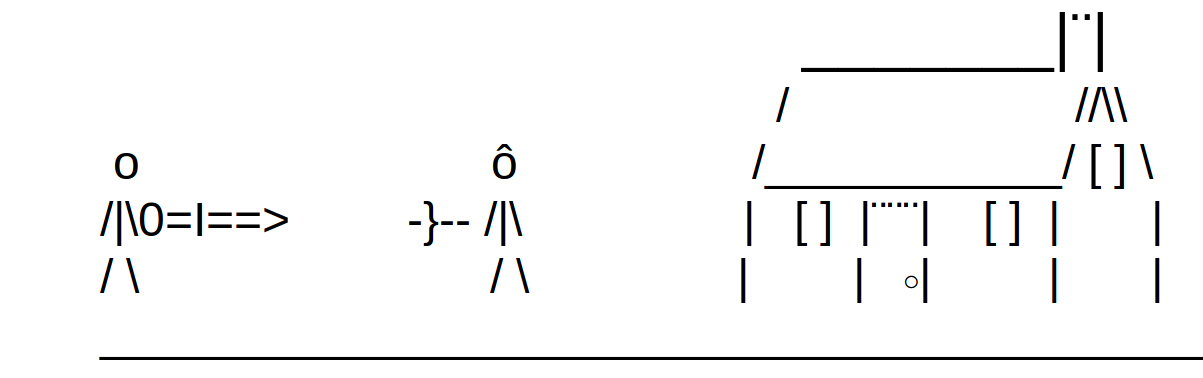
\includegraphics[width=\linewidth]{Visual.png}
\end{figure}
  
\section{Kravformulering}
\subsection{Spelmeny}
\textbf{SKA:}

1. Har alternativ för att påbörja en spelomgång samt för att avsluta spelet.

\textbf{BÖR:}

2. Ha ett alternativ för att komma till en highscore lista som listar de 3 bästa highscoren.

\sout{3. Vara visuellt tilltalande.}
\subsection{Spelkaraktär}
\textbf{SKA:}

4. Spelarkaraktären kontrolleras enligt avsnitt 1.4 samt 1.5.2.

5. Spelarkaraktären har två olika typer av attacker som kontrolleras enligt tabellen i avsnitt 1.4.

6. Ha olika visuella representation för de olika attackerna.

7. Spelarkaraktären har total tre liv som representeras i form av hjärtan på skärmen.

8. Spelarkaraktären tar ett livs skada vid kollision med fiende.

9. När spelarkaraktären tar skada blir denne immun mot att ta mer skada i 2 sekunder. 

11. När antal liv är slut avslutas spelet och en game over skärm visas.

\textbf{BÖR:}

5. Spelarkaraktären har tre olika typer av attacker som kontrolleras enligt tabellen i avsnitt 1.4.

10. Spelarkaraktären ändrar färg när denne tar skada.

12. Ha en viss chans att yttra ett ljud vid en attack. Olika attacker är kopplade till olika ljud. 10\% chans att producera ett ljud vid attack.

13. Spelarkaraktären ska kunna parera attacker genom att spelaren håller inne en tangent. Pareringen innebär att spelarkaraktären inte kan ta skada av fiendeattacker som sker från riktningen spelarakaraktären är vänd.

14. Spelarkaraktären ändrar färg under tiden denne är immun mot skada.

15. Visa en dödsanimering när spelarkaraktären når 0 liv.
\subsection{Fiender}
\textbf{SKA:}

16. Bönder och riddare följer spelarkaraktären.

19. Riddare besegras och försvinner efter de träffats av två hårda attacker.

20. Bönder och riddare fortsätter attackera spelarkaraktären tills de är besegrade eller spelarkaraktären dör.

\textbf{BÖR:}

17. Bönderna har två varianter av sitt vapen och vilket vapen de har är slumpgenererat.

18. Bönder och byfånar besegras och försvinner när spelarkaraktären utför korrekt attack.

21. Byfånen skickas in, korsar hela spelplanen samt lämnar den på motsatt sida såvida spelarkaraktären inte besegrar den. Även om byfånen skadar spelarkaraktären fortsätter den på sin bestämda väg.

22. Implementera boss som sista fiende i spelet.

23. Ha en dödsanimering för de olika fienderna.

24. Riddare förlorar först sin rustning och besegras av slaget efter att deras rustning försvunnit.
\subsection{Spelplan}
\textbf{SKA:}

25. Ha fasta barriärer spelarkaraktären inte kan passera. 

26. Fiender ska skickas in i bestämda tidsintervall.

27. När en fiende besegras uppdateras poängen.

28. När spelaren förlorar visas en game over-skärm med spelarens poängrekord.

29. Vid vinst visas poängrekord samt en vinstskärm.

30. 2D-grafik.

31. Spelplanen är statisk (ingen scrollning sker).

32. Spelplan laddas in från fil. Varje spelplan har ett eget mönster av fiendegenerering.

\textbf{BÖR:}

33. Vid spelets start visas en sekvens där spelets bakgrundshistoria presenteras.

34. Vid vinst visas en sekvens av vad som händer efter spelarkaraktären besegrat hela byn.

35. Inskickandet av fiender är delvis slumpgenererat.

36. Automatisk anpassning till fönstrets storlek.

\subsection{Kravuppfyllelse}
Krav hämtas från kursens kurshemsida och är utformade av kursledningen.

\textit{Spelet ska simulera en värld som innehåller olika typer av objekt. Objekten ska ha olika beteenden och röra sig i världen och agera på olika sätt när de möter andra objekt.}

\textbf{Uppfylls av krav 4, 5, 8, 9, 10, 16, 17, 18, 19, 20, 21, 25 och 26.}

\textit{Det måste finnas minst tre olika typer av objekt och det ska finnas flera instanser av minst två av dessa. T.ex ett spelarobjekt och många instanser av två olika slags fiendeobjekt.}

\textbf{Uppfylls genom implementation av spelkaraktär och fiender samt krav 26.}

\textit{Ett beteende som måste finnas med är att figurerna ska röra sig över skärmen. Rörelsen kan följa ett mönster och/eller vara slumpmässig. Minst ett objekt, utöver spelaren ska ha någon typ av rörelse.}

\textbf{Uppfylls av krav 16 och 21.}

\textit{En figur ska styras av spelaren, antingen med tangentbordet eller med musen. Du kan även göra ett spel där man spelar två stycken genom att dela på tangentbordet (varje spelare använder olika tangenter). Då styr man var sin figur.}

\textbf{Uppfylls av krav 4 och 5.}

\textit{Grafiken ska vara tvådimensionell.}

\textbf{Uppfylls av krav 30.}

\textit{Världen (spelplanen) kan antas vara lika stor som fönstret (du kan göra en större spelplan med scrollning, men det blir lite krångligare).}

\textbf{Uppfylls av krav 31.}

\textit{Det ska finnas kollisionshantering, det vill säga, det ska hända olika saker när objekten möter varandra, de ska påverka varandra på något sätt. T.ex kan ett av objekten tas bort, eller så kan objekten förvandlas på något sätt, eller så kan ett nytt objekt skapas. (...)}

\textbf{Uppfylls av krav 8, 9, 10, 18, 19 och 21.}

\textit{Det ska vara enkelt att lägga till eller ändra banor i spelet (...).}

\textbf{Uppfylls av krav 31.}

\textit{Spelet måste upplevas som ett sammanhängande spel som går att spela!}

\textbf{Uppfylls av krav 1, 11, 27, 28 och 29.}

\end{document}
